\SourceLeaf{406}%
tiver Werth seine gute verschiedene Bedeutung haben, und der Begriff der Area muss also so festgesetzt werden, dass diess klar einleuchte. Allein dann muss man noch einen Schritt weiter gehen und Figuren betrachten, deren Umfang sich selbst einmal oder mehreremale schneidet, z. B.
\begin{center}
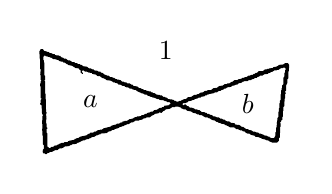
\begin{tikzpicture}[x=.00225in,y=-.00225in]
\path[use as bounding box] (0,0) rectangle (616,308);
\path[fill=black,even odd rule] (26,53) -- (27,70) -- (28,71) -- (28,92) -- (29,93) -- (28,105) -- (29,106) -- (29,116) -- (31,118) -- (29,120) -- (29,124) -- (28,125) -- (28,130) -- (29,131) -- (29,157) -- (31,158) -- (31,159) -- (29,161) -- (29,168) -- (28,169) -- (28,171) -- (31,173) -- (32,192) -- (34,194) -- (34,196) -- (33,197) -- (33,206) -- (32,207) -- (32,214) -- (33,215) -- (33,225) -- (32,226) -- (32,229) -- (33,230) -- (33,240) -- (34,241) -- (34,260) -- (36,262) -- (36,270) -- (34,272) -- (34,274) -- (33,275) -- (34,276) -- (34,279) -- (35,280) -- (38,280) -- (40,282) -- (42,282) -- (45,279) -- (47,279) -- (50,277) -- (55,277) -- (56,275) -- (58,275) -- (61,273) -- (66,273) -- (71,269) -- (76,269) -- (80,267) -- (82,265) -- (92,264) -- (95,262) -- (97,262) -- (99,260) -- (108,259) -- (112,256) -- (114,256) -- (115,255) -- (117,255) -- (119,253) -- (121,253) -- (123,251) -- (127,251) -- (130,249) -- (137,248) -- (138,246) -- (141,246) -- (143,244) -- (149,243) -- (153,240) -- (155,240) -- (159,238) -- (162,238) -- (163,236) -- (176,235) -- (181,231) -- (184,231) -- (189,228) -- (192,228) -- (194,226) -- (202,224) -- (206,221) -- (209,221) -- (210,220) -- (215,219) -- (216,217) -- (218,217) -- (222,215) -- (225,215) -- (231,211) -- (235,211) -- (237,209) -- (239,209) -- (240,207) -- (248,207) -- (249,206) -- (255,205) -- (259,202) -- (262,202) -- (265,200) -- (272,200) -- (277,196) -- (280,195) -- (284,192) -- (291,191) -- (295,188) -- (297,190) -- (298,190) -- (302,186) -- (305,185) -- (308,182) -- (316,181) -- (317,180) -- (319,180) -- (322,177) -- (328,177) -- (329,176) -- (336,176) -- (337,177) -- (340,177) -- (342,179) -- (342,180) -- (344,180) -- (348,182) -- (352,182) -- (355,185) -- (365,187) -- (369,190) -- (375,191) -- (378,193) -- (381,193) -- (383,195) -- (388,195) -- (396,200) -- (401,200) -- (404,202) -- (406,202) -- (408,204) -- (412,206) -- (417,207) -- (421,210) -- (423,210) -- (426,212) -- (429,212) -- (431,214) -- (438,215) -- (440,217) -- (443,217) -- (444,219) -- (446,219) -- (451,222) -- (460,222) -- (465,226) -- (469,226) -- (471,228) -- (473,228) -- (474,229) -- (478,229) -- (480,231) -- (483,231) -- (486,234) -- (490,236) -- (494,236) -- (498,239) -- (506,241) -- (507,243) -- (515,244) -- (516,245) -- (521,246) -- (522,248) -- (525,248) -- (526,249) -- (529,249) -- (533,251) -- (536,251) -- (538,253) -- (545,256) -- (556,256) -- (560,252) -- (560,246) -- (562,245) -- (562,235) -- (563,234) -- (563,221) -- (564,220) -- (564,214) -- (563,213) -- (563,211) -- (565,209) -- (565,207) -- (568,205) -- (568,199) -- (569,198) -- (569,186) -- (570,185) -- (570,177) -- (572,175) -- (572,165) -- (573,164) -- (573,158) -- (574,157) -- (574,148) -- (576,146) -- (574,144) -- (574,142) -- (576,140) -- (576,129) -- (579,123) -- (579,115) -- (581,113) -- (581,98) -- (582,97) -- (582,91) -- (583,90) -- (583,83) -- (580,79) -- (574,79) -- (570,82) -- (560,83) -- (558,85) -- (554,87) -- (548,88) -- (546,90) -- (542,90) -- (541,91) -- (538,91) -- (537,92) -- (534,92) -- (533,93) -- (529,93) -- (524,97) -- (515,97) -- (511,101) -- (508,101) -- (506,103) -- (504,103) -- (502,105) -- (499,105) -- (495,107) -- (492,107) -- (488,110) -- (485,110) -- (481,112) -- (478,112) -- (476,114) -- (470,115) -- (467,117) -- (461,117) -- (456,121) -- (454,121) -- (450,124) -- (446,124) -- (443,126) -- (439,126) -- (435,129) -- (428,130) -- (424,132) -- (422,134) -- (414,135) -- (409,139) -- (402,139) -- (399,141) -- (395,141) -- (391,144) -- (385,145) -- (381,148) -- (379,148) -- (375,150) -- (371,150) -- (365,154) -- (363,154) -- (362,155) -- (357,155) -- (354,158) -- (352,159) -- (349,159) -- (346,161) -- (344,161) -- (342,163) -- (339,163) -- (335,165) -- (332,165) -- (330,163) -- (327,163) -- (325,161) -- (323,161) -- (322,160) -- (317,160) -- (316,159) -- (313,159) -- (310,156) -- (308,156) -- (305,154) -- (302,154) -- (299,151) -- (295,151) -- (294,150) -- (290,150) -- (289,149) -- (287,149) -- (283,146) -- (280,146) -- (278,144) -- (276,144) -- (274,142) -- (270,142) -- (269,141) -- (266,141) -- (263,139) -- (259,139) -- (257,137) -- (255,137) -- (252,135) -- (249,135) -- (244,131) -- (236,130) -- (234,128) -- (234,127) -- (231,127) -- (227,124) -- (222,124) -- (220,122) -- (216,122) -- (213,120) -- (210,120) -- (207,117) -- (205,117) -- (204,116) -- (200,116) -- (199,115) -- (195,114) -- (193,112) -- (191,112) -- (187,110) -- (184,110) -- (180,107) -- (177,107) -- (174,105) -- (172,105) -- (167,101) -- (163,100) -- (162,98) -- (158,98) -- (155,96) -- (151,96) -- (150,95) -- (148,95) -- (147,93) -- (144,93) -- (141,91) -- (137,91) -- (132,87) -- (124,86) -- (120,83) -- (118,83) -- (116,81) -- (112,81) -- (110,79) -- (106,79) -- (104,77) -- (100,77) -- (94,73) -- (90,73) -- (85,69) -- (81,69) -- (79,67) -- (75,66) -- (73,64) -- (73,63) -- (70,63) -- (69,62) -- (64,62) -- (63,61) -- (61,61) -- (60,59) -- (57,59) -- (53,57) -- (50,57) -- (46,54) -- (43,54) -- (42,53) -- (37,52) -- (34,48) -- (29,48) -- cycle (575,91) -- (575,94) -- (574,95) -- (574,100) -- (572,101) -- (572,109) -- (570,112) -- (570,126) -- (567,129) -- (567,134) -- (566,135) -- (566,139) -- (565,140) -- (565,148) -- (564,149) -- (564,161) -- (562,163) -- (562,168) -- (561,169) -- (561,179) -- (560,180) -- (560,187) -- (559,188) -- (559,199) -- (557,201) -- (556,211) -- (555,212) -- (556,216) -- (555,217) -- (555,222) -- (554,223) -- (554,232) -- (552,234) -- (552,241) -- (551,242) -- (551,244) -- (549,246) -- (543,246) -- (542,245) -- (540,245) -- (539,243) -- (536,243) -- (533,241) -- (527,240) -- (525,238) -- (523,238) -- (519,236) -- (516,236) -- (514,234) -- (508,233) -- (507,232) -- (503,232) -- (499,229) -- (493,228) -- (491,226) -- (487,226) -- (480,221) -- (477,221) -- (472,217) -- (463,216) -- (461,213) -- (453,212) -- (449,209) -- (445,209) -- (441,207) -- (439,205) -- (436,205) -- (433,203) -- (430,203) -- (426,200) -- (422,200) -- (418,198) -- (414,198) -- (411,195) -- (406,194) -- (404,192) -- (400,192) -- (399,190) -- (397,190) -- (393,188) -- (388,188) -- (383,184) -- (380,184) -- (377,182) -- (373,182) -- (371,180) -- (367,179) -- (366,178) -- (361,178) -- (358,175) -- (356,175) -- (352,171) -- (350,171) -- (348,173) -- (347,173) -- (345,171) -- (345,170) -- (347,168) -- (352,168) -- (353,167) -- (355,167) -- (358,164) -- (364,163) -- (368,161) -- (371,161) -- (373,159) -- (378,158) -- (381,156) -- (385,156) -- (387,154) -- (394,153) -- (396,151) -- (399,151) -- (400,149) -- (403,149) -- (404,148) -- (415,146) -- (417,144) -- (422,144) -- (426,141) -- (430,141) -- (432,139) -- (436,138) -- (438,136) -- (441,136) -- (445,133) -- (453,132) -- (457,129) -- (460,129) -- (464,127) -- (467,127) -- (470,124) -- (476,123) -- (480,120) -- (482,120) -- (483,119) -- (490,119) -- (493,117) -- (498,117) -- (500,115) -- (504,114) -- (507,112) -- (511,112) -- (512,110) -- (516,109) -- (518,107) -- (523,107) -- (527,104) -- (535,103) -- (537,101) -- (540,101) -- (542,99) -- (546,98) -- (550,95) -- (555,95) -- (556,94) -- (559,94) -- (565,90) -- (569,90) -- (570,89) -- (573,89) -- cycle (35,65) -- (38,62) -- (39,62) -- (41,64) -- (44,64) -- (45,65) -- (48,65) -- (51,67) -- (53,67) -- (57,70) -- (62,70) -- (63,71) -- (68,72) -- (72,75) -- (79,76) -- (80,78) -- (83,78) -- (87,81) -- (89,81) -- (90,83) -- (99,85) -- (107,90) -- (111,90) -- (112,91) -- (114,91) -- (115,93) -- (118,95) -- (118,100) -- (122,103) -- (123,103) -- (123,101) -- (121,99) -- (121,97) -- (123,95) -- (126,96) -- (128,98) -- (132,98) -- (136,100) -- (143,101) -- (144,103) -- (146,103) -- (147,104) -- (151,104) -- (156,108) -- (161,108) -- (166,112) -- (170,113) -- (174,115) -- (176,117) -- (185,118) -- (189,120) -- (191,122) -- (194,122) -- (195,123) -- (200,124) -- (202,126) -- (202,127) -- (207,127) -- (212,130) -- (216,130) -- (217,132) -- (219,132) -- (220,133) -- (224,133) -- (228,136) -- (232,136) -- (235,138) -- (241,139) -- (243,141) -- (249,144) -- (251,144) -- (253,146) -- (258,147) -- (261,149) -- (265,149) -- (268,152) -- (270,152) -- (274,154) -- (277,154) -- (279,156) -- (282,156) -- (289,159) -- (293,159) -- (294,161) -- (304,162) -- (306,164) -- (309,164) -- (311,166) -- (316,166) -- (319,169) -- (314,173) -- (305,174) -- (303,177) -- (300,177) -- (298,179) -- (294,179) -- (288,183) -- (282,184) -- (279,187) -- (275,187) -- (272,189) -- (267,190) -- (265,192) -- (262,192) -- (258,195) -- (254,195) -- (252,197) -- (250,197) -- (249,198) -- (244,198) -- (243,199) -- (238,200) -- (234,203) -- (232,203) -- (231,204) -- (227,204) -- (221,208) -- (216,208) -- (215,209) -- (212,209) -- (211,211) -- (206,212) -- (204,214) -- (199,214) -- (197,216) -- (194,216) -- (193,217) -- (188,218) -- (184,221) -- (178,222) -- (177,223) -- (174,223) -- (173,224) -- (170,224) -- (166,227) -- (162,227) -- (161,228) -- (155,229) -- (153,231) -- (151,232) -- (148,232) -- (146,234) -- (140,234) -- (137,237) -- (135,237) -- (131,240) -- (117,243) -- (113,246) -- (110,246) -- (107,248) -- (105,248) -- (104,250) -- (93,252) -- (92,253) -- (90,253) -- (89,255) -- (82,255) -- (80,257) -- (75,257) -- (74,258) -- (72,258) -- (70,260) -- (68,260) -- (66,262) -- (60,263) -- (58,265) -- (56,266) -- (53,266) -- (49,269) -- (44,265) -- (44,236) -- (42,234) -- (42,226) -- (44,225) -- (44,223) -- (42,222) -- (42,214) -- (41,213) -- (41,205) -- (42,204) -- (41,192) -- (42,191) -- (42,189) -- (41,188) -- (40,148) -- (39,147) -- (39,120) -- (37,118) -- (39,116) -- (39,108) -- (37,106) -- (37,78) -- (36,77) -- (36,73) -- (35,72) -- cycle;
\node[inner sep=0pt,font=\normalsize] at (308,51) {$1$};
\node[inner sep=0pt,font=\normalsize] at (140,165) {$a$};
\node[inner sep=0pt,font=\normalsize] at (491,169) {$b$};
\end{tikzpicture}
\quad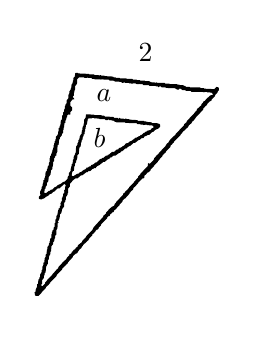
\begin{tikzpicture}[x=.00225in,y=-.00225in]
\path[use as bounding box] (0,0) rectangle (455,630);
\path[fill=black,even odd rule] (425,133) -- (421,132) -- (416,137) -- (394,136) -- (393,135) -- (386,135) -- (384,133) -- (362,133) -- (361,132) -- (353,132) -- (351,130) -- (348,130) -- (347,128) -- (339,128) -- (338,127) -- (334,127) -- (333,126) -- (317,126) -- (316,125) -- (307,125) -- (305,123) -- (289,123) -- (288,122) -- (284,123) -- (283,122) -- (276,122) -- (275,121) -- (273,121) -- (271,119) -- (262,119) -- (261,118) -- (251,118) -- (250,117) -- (244,117) -- (243,116) -- (235,116) -- (233,114) -- (221,114) -- (220,113) -- (206,113) -- (205,112) -- (197,112) -- (196,111) -- (192,111) -- (190,109) -- (172,108) -- (171,107) -- (164,107) -- (163,106) -- (161,106) -- (160,107) -- (158,106) -- (149,106) -- (148,104) -- (137,104) -- (136,103) -- (113,102) -- (112,101) -- (107,101) -- (106,102) -- (105,109) -- (102,112) -- (102,117) -- (101,118) -- (101,121) -- (100,122) -- (100,124) -- (98,126) -- (97,135) -- (96,136) -- (96,138) -- (93,142) -- (93,146) -- (91,150) -- (91,157) -- (87,162) -- (87,168) -- (84,172) -- (84,174) -- (83,175) -- (83,180) -- (81,184) -- (81,187) -- (79,189) -- (79,194) -- (77,196) -- (77,202) -- (76,203) -- (76,205) -- (74,207) -- (73,217) -- (71,220) -- (71,223) -- (69,224) -- (69,231) -- (68,232) -- (68,236) -- (66,240) -- (63,243) -- (63,248) -- (62,249) -- (62,252) -- (60,254) -- (60,257) -- (59,258) -- (59,261) -- (58,262) -- (58,267) -- (57,268) -- (57,271) -- (55,273) -- (55,276) -- (54,277) -- (54,280) -- (52,282) -- (52,285) -- (50,286) -- (50,290) -- (49,291) -- (49,299) -- (47,302) -- (47,307) -- (45,309) -- (44,315) -- (43,316) -- (43,319) -- (40,322) -- (39,333) -- (37,336) -- (37,339) -- (35,340) -- (35,345) -- (34,346) -- (33,353) -- (31,355) -- (31,359) -- (28,365) -- (28,371) -- (29,373) -- (25,377) -- (25,381) -- (26,382) -- (31,383) -- (34,381) -- (36,381) -- (41,377) -- (45,375) -- (49,371) -- (53,370) -- (57,366) -- (60,365) -- (66,359) -- (68,358) -- (71,358) -- (81,349) -- (83,349) -- (85,351) -- (85,352) -- (84,353) -- (83,361) -- (81,363) -- (82,367) -- (79,371) -- (79,375) -- (78,376) -- (78,378) -- (76,380) -- (76,387) -- (74,388) -- (74,391) -- (73,392) -- (74,396) -- (72,398) -- (72,401) -- (70,403) -- (69,403) -- (69,406) -- (68,407) -- (66,418) -- (64,420) -- (64,425) -- (62,428) -- (62,435) -- (60,436) -- (60,444) -- (58,446) -- (58,450) -- (55,453) -- (55,455) -- (54,456) -- (54,460) -- (53,461) -- (53,468) -- (51,470) -- (50,470) -- (50,475) -- (49,476) -- (49,479) -- (47,482) -- (47,485) -- (44,489) -- (44,494) -- (43,495) -- (42,504) -- (40,506) -- (40,511) -- (38,514) -- (37,523) -- (35,524) -- (35,529) -- (33,533) -- (33,539) -- (31,541) -- (31,545) -- (28,550) -- (28,556) -- (26,557) -- (26,560) -- (24,562) -- (23,571) -- (21,572) -- (21,577) -- (18,584) -- (18,588) -- (15,591) -- (16,593) -- (16,596) -- (18,598) -- (24,598) -- (31,591) -- (31,590) -- (40,581) -- (41,578) -- (44,575) -- (45,575) -- (49,570) -- (50,570) -- (50,568) -- (64,554) -- (65,551) -- (77,539) -- (77,537) -- (83,531) -- (84,531) -- (84,530) -- (88,526) -- (89,526) -- (90,523) -- (101,511) -- (101,509) -- (107,504) -- (110,503) -- (115,495) -- (120,491) -- (120,489) -- (123,486) -- (123,485) -- (135,474) -- (138,469) -- (144,463) -- (144,461) -- (146,459) -- (147,459) -- (150,455) -- (151,455) -- (151,453) -- (154,450) -- (156,450) -- (158,448) -- (158,446) -- (163,441) -- (164,438) -- (177,425) -- (177,423) -- (180,420) -- (182,420) -- (183,419) -- (183,417) -- (185,415) -- (186,415) -- (188,412) -- (190,412) -- (192,410) -- (192,408) -- (194,406) -- (195,406) -- (204,396) -- (205,396) -- (205,394) -- (211,388) -- (212,385) -- (216,381) -- (217,381) -- (227,370) -- (227,368) -- (229,367) -- (230,365) -- (235,361) -- (236,357) -- (242,352) -- (242,351) -- (246,347) -- (246,346) -- (256,336) -- (258,336) -- (260,334) -- (260,330) -- (262,328) -- (263,328) -- (267,323) -- (270,322) -- (274,318) -- (274,316) -- (277,313) -- (278,313) -- (278,312) -- (282,308) -- (282,307) -- (290,299) -- (290,298) -- (294,294) -- (294,293) -- (300,287) -- (300,285) -- (302,284) -- (302,283) -- (306,279) -- (307,279) -- (309,275) -- (318,266) -- (319,262) -- (321,261) -- (325,256) -- (326,256) -- (326,254) -- (341,239) -- (341,238) -- (345,234) -- (345,233) -- (357,222) -- (360,217) -- (365,213) -- (367,209) -- (369,208) -- (373,203) -- (374,203) -- (374,201) -- (391,183) -- (392,179) -- (394,178) -- (395,176) -- (400,172) -- (400,170) -- (406,164) -- (408,164) -- (410,162) -- (410,160) -- (418,152) -- (418,150) -- (423,145) -- (424,142) -- (426,140) -- (426,134) -- cycle (98,329) -- (99,323) -- (100,321) -- (102,319) -- (103,319) -- (104,309) -- (105,308) -- (105,305) -- (106,304) -- (106,302) -- (108,300) -- (108,297) -- (110,293) -- (110,290) -- (111,289) -- (111,284) -- (114,281) -- (115,269) -- (116,268) -- (116,266) -- (118,265) -- (119,256) -- (120,255) -- (120,252) -- (122,250) -- (123,243) -- (125,241) -- (125,238) -- (127,237) -- (127,232) -- (128,231) -- (128,226) -- (129,225) -- (130,217) -- (132,215) -- (134,204) -- (136,202) -- (143,202) -- (144,201) -- (147,201) -- (148,202) -- (155,202) -- (156,203) -- (160,203) -- (161,204) -- (172,204) -- (174,206) -- (178,206) -- (180,204) -- (182,206) -- (187,206) -- (188,207) -- (191,207) -- (195,210) -- (197,210) -- (198,211) -- (217,211) -- (218,212) -- (225,212) -- (226,213) -- (243,213) -- (245,215) -- (251,215) -- (252,216) -- (257,216) -- (258,217) -- (265,216) -- (266,217) -- (270,217) -- (271,218) -- (278,218) -- (281,221) -- (281,222) -- (279,224) -- (277,224) -- (274,228) -- (266,230) -- (265,232) -- (263,232) -- (261,234) -- (258,235) -- (254,239) -- (252,239) -- (250,242) -- (248,242) -- (243,245) -- (241,245) -- (232,252) -- (227,254) -- (224,257) -- (219,258) -- (215,263) -- (212,264) -- (210,266) -- (206,268) -- (204,268) -- (202,271) -- (198,272) -- (194,276) -- (192,277) -- (188,277) -- (181,283) -- (179,283) -- (178,285) -- (175,285) -- (169,290) -- (167,290) -- (165,292) -- (161,293) -- (157,297) -- (156,297) -- (156,298) -- (154,300) -- (152,300) -- (146,305) -- (142,306) -- (140,309) -- (138,309) -- (134,312) -- (131,312) -- (131,313) -- (128,316) -- (125,317) -- (119,322) -- (116,322) -- (116,323) -- (114,325) -- (110,326) -- (102,331) -- (100,331) -- cycle (410,145) -- (413,148) -- (413,149) -- (412,150) -- (407,151) -- (402,156) -- (401,156) -- (394,164) -- (393,164) -- (391,166) -- (391,167) -- (387,171) -- (387,173) -- (377,182) -- (377,184) -- (373,188) -- (373,189) -- (355,208) -- (354,211) -- (349,215) -- (348,218) -- (330,237) -- (330,238) -- (318,249) -- (318,250) -- (315,253) -- (315,255) -- (310,259) -- (307,264) -- (292,280) -- (292,281) -- (286,286) -- (286,287) -- (282,291) -- (282,293) -- (280,295) -- (280,296) -- (273,303) -- (271,303) -- (270,302) -- (268,303) -- (268,308) -- (251,326) -- (251,327) -- (246,332) -- (246,334) -- (241,339) -- (241,340) -- (237,344) -- (237,345) -- (226,356) -- (226,357) -- (222,361) -- (222,362) -- (220,363) -- (217,366) -- (217,367) -- (213,370) -- (213,372) -- (197,389) -- (197,390) -- (194,393) -- (193,396) -- (191,398) -- (188,399) -- (180,406) -- (180,407) -- (175,412) -- (174,415) -- (169,419) -- (168,422) -- (147,445) -- (144,451) -- (132,463) -- (129,468) -- (122,475) -- (121,478) -- (112,485) -- (112,487) -- (109,490) -- (108,490) -- (107,492) -- (104,495) -- (103,495) -- (99,500) -- (98,500) -- (98,502) -- (96,504) -- (93,505) -- (93,507) -- (88,512) -- (86,516) -- (76,525) -- (76,526) -- (69,533) -- (68,536) -- (65,539) -- (64,539) -- (64,540) -- (55,550) -- (55,551) -- (43,563) -- (43,564) -- (39,568) -- (39,570) -- (33,576) -- (32,576) -- (30,574) -- (30,573) -- (32,571) -- (32,563) -- (36,558) -- (36,553) -- (38,551) -- (38,547) -- (40,545) -- (41,533) -- (43,530) -- (43,528) -- (45,527) -- (45,519) -- (47,516) -- (48,508) -- (50,507) -- (51,499) -- (52,498) -- (52,493) -- (53,492) -- (53,487) -- (57,482) -- (57,478) -- (59,476) -- (60,470) -- (61,469) -- (61,464) -- (64,461) -- (64,451) -- (66,448) -- (66,445) -- (67,444) -- (67,436) -- (69,435) -- (67,431) -- (70,429) -- (70,426) -- (71,425) -- (71,422) -- (72,421) -- (72,416) -- (75,413) -- (77,404) -- (81,399) -- (81,391) -- (84,387) -- (84,384) -- (85,383) -- (85,378) -- (89,372) -- (89,369) -- (90,368) -- (90,359) -- (94,354) -- (94,349) -- (95,347) -- (99,343) -- (99,342) -- (105,337) -- (107,336) -- (111,336) -- (119,329) -- (122,329) -- (131,322) -- (134,322) -- (135,320) -- (138,320) -- (140,319) -- (144,315) -- (146,315) -- (148,313) -- (152,313) -- (152,312) -- (156,308) -- (159,307) -- (169,299) -- (172,299) -- (179,293) -- (182,293) -- (182,292) -- (185,289) -- (187,289) -- (190,286) -- (192,285) -- (196,285) -- (204,279) -- (206,279) -- (208,276) -- (210,276) -- (218,269) -- (221,269) -- (223,266) -- (224,266) -- (226,264) -- (228,264) -- (236,257) -- (239,257) -- (248,250) -- (250,250) -- (253,247) -- (255,246) -- (258,246) -- (261,242) -- (263,242) -- (268,239) -- (271,239) -- (277,233) -- (280,232) -- (284,228) -- (291,225) -- (295,221) -- (295,216) -- (293,214) -- (290,214) -- (289,213) -- (278,213) -- (276,211) -- (265,210) -- (264,209) -- (260,209) -- (259,208) -- (246,208) -- (244,206) -- (227,205) -- (226,204) -- (221,204) -- (220,203) -- (217,203) -- (216,204) -- (214,203) -- (207,203) -- (205,201) -- (203,203) -- (202,203) -- (200,201) -- (193,201) -- (191,199) -- (172,198) -- (170,196) -- (165,196) -- (164,195) -- (149,195) -- (148,194) -- (131,193) -- (130,194) -- (130,198) -- (129,199) -- (129,201) -- (126,205) -- (126,213) -- (125,214) -- (125,218) -- (123,220) -- (123,222) -- (122,223) -- (122,228) -- (121,229) -- (121,232) -- (120,233) -- (120,237) -- (118,239) -- (116,243) -- (116,246) -- (115,247) -- (115,249) -- (113,251) -- (113,255) -- (111,258) -- (111,261) -- (108,265) -- (107,279) -- (105,282) -- (105,284) -- (103,286) -- (102,294) -- (101,295) -- (101,299) -- (100,300) -- (100,303) -- (98,305) -- (98,309) -- (97,310) -- (97,313) -- (96,314) -- (96,319) -- (92,324) -- (92,329) -- (89,333) -- (89,336) -- (88,338) -- (83,343) -- (79,344) -- (74,348) -- (67,351) -- (63,355) -- (61,355) -- (55,361) -- (52,361) -- (49,364) -- (47,364) -- (42,368) -- (38,369) -- (37,368) -- (38,360) -- (40,358) -- (40,355) -- (43,351) -- (43,346) -- (46,342) -- (47,333) -- (51,327) -- (52,318) -- (55,315) -- (55,310) -- (56,309) -- (56,306) -- (57,305) -- (57,299) -- (59,297) -- (59,291) -- (61,289) -- (61,287) -- (63,285) -- (64,285) -- (64,281) -- (66,277) -- (66,267) -- (67,266) -- (67,262) -- (69,261) -- (70,250) -- (72,247) -- (72,245) -- (76,240) -- (76,237) -- (79,234) -- (79,228) -- (80,227) -- (80,223) -- (81,222) -- (82,213) -- (84,212) -- (84,208) -- (86,204) -- (86,201) -- (88,199) -- (88,196) -- (91,193) -- (92,194) -- (94,194) -- (95,193) -- (95,188) -- (99,184) -- (99,178) -- (95,174) -- (95,166) -- (100,160) -- (103,160) -- (104,159) -- (101,155) -- (101,153) -- (103,151) -- (103,145) -- (104,144) -- (104,141) -- (106,137) -- (106,130) -- (108,128) -- (110,124) -- (110,115) -- (114,111) -- (126,111) -- (127,112) -- (132,112) -- (134,111) -- (135,112) -- (142,112) -- (144,114) -- (148,114) -- (149,115) -- (162,115) -- (163,116) -- (165,115) -- (169,115) -- (170,116) -- (181,116) -- (183,118) -- (191,118) -- (195,120) -- (204,120) -- (205,121) -- (208,121) -- (211,123) -- (213,123) -- (215,121) -- (217,123) -- (225,123) -- (226,124) -- (230,124) -- (231,125) -- (234,125) -- (235,124) -- (240,124) -- (244,126) -- (249,126) -- (250,125) -- (251,126) -- (256,126) -- (258,128) -- (270,128) -- (272,130) -- (285,130) -- (286,131) -- (290,131) -- (292,133) -- (294,131) -- (297,131) -- (299,133) -- (307,133) -- (308,134) -- (312,134) -- (313,135) -- (328,135) -- (329,136) -- (331,136) -- (333,138) -- (337,138) -- (338,136) -- (341,136) -- (345,139) -- (351,139) -- (353,141) -- (363,141) -- (365,143) -- (390,143) -- (391,144) -- (399,143) -- (400,144) -- (406,144) -- (407,145) -- cycle;
\node[inner sep=0pt,font=\normalsize] at (263,56) {$2$};
\node[inner sep=0pt,font=\normalsize] at (170,151) {$a$};
\node[inner sep=0pt,font=\normalsize] at (160,245) {$b$};
\end{tikzpicture}
\quad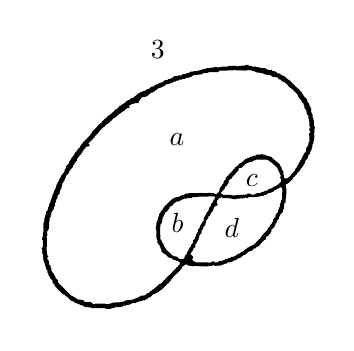
\begin{tikzpicture}[x=.00225in,y=-.00225in]
\path[use as bounding box] (0,0) rectangle (665,658);
\path[fill=black,even odd rule] (606,138) -- (605,138) -- (604,136) -- (602,136) -- (600,134) -- (600,133) -- (598,132) -- (595,129) -- (595,128) -- (593,127) -- (590,124) -- (590,123) -- (585,119) -- (584,117) -- (582,117) -- (572,108) -- (566,106) -- (561,102) -- (557,102) -- (554,99) -- (550,97) -- (547,97) -- (543,94) -- (535,94) -- (533,92) -- (531,92) -- (529,90) -- (520,90) -- (519,89) -- (515,89) -- (514,88) -- (510,88) -- (509,87) -- (500,87) -- (499,85) -- (494,85) -- (490,83) -- (486,83) -- (483,85) -- (481,85) -- (480,84) -- (478,85) -- (470,85) -- (468,87) -- (466,85) -- (448,85) -- (446,87) -- (433,87) -- (432,88) -- (426,88) -- (425,89) -- (423,89) -- (422,88) -- (416,88) -- (415,89) -- (408,89) -- (407,90) -- (399,90) -- (397,92) -- (392,92) -- (388,94) -- (384,94) -- (383,96) -- (379,96) -- (378,97) -- (370,97) -- (369,98) -- (363,98) -- (360,101) -- (356,101) -- (353,103) -- (345,104) -- (344,106) -- (342,106) -- (341,107) -- (337,106) -- (334,108) -- (327,108) -- (322,112) -- (318,114) -- (315,114) -- (311,117) -- (306,117) -- (300,122) -- (294,123) -- (292,125) -- (284,128) -- (281,131) -- (275,132) -- (270,137) -- (267,137) -- (261,141) -- (258,141) -- (255,143) -- (252,143) -- (250,145) -- (246,147) -- (241,152) -- (239,152) -- (239,153) -- (236,156) -- (234,157) -- (231,157) -- (227,161) -- (223,162) -- (215,169) -- (214,169) -- (212,171) -- (210,171) -- (208,174) -- (205,174) -- (204,176) -- (198,182) -- (196,182) -- (190,189) -- (189,189) -- (183,195) -- (181,195) -- (173,203) -- (172,203) -- (165,210) -- (165,212) -- (161,214) -- (143,233) -- (143,235) -- (139,239) -- (139,240) -- (123,256) -- (123,257) -- (119,261) -- (116,267) -- (111,272) -- (111,273) -- (105,280) -- (105,281) -- (103,283) -- (103,285) -- (98,290) -- (97,293) -- (93,298) -- (92,302) -- (85,310) -- (85,313) -- (84,314) -- (84,316) -- (82,318) -- (82,321) -- (74,331) -- (73,335) -- (70,338) -- (69,343) -- (66,346) -- (66,348) -- (64,351) -- (63,358) -- (61,359) -- (61,361) -- (59,363) -- (59,365) -- (58,366) -- (58,369) -- (55,373) -- (55,376) -- (53,380) -- (53,383) -- (51,385) -- (51,388) -- (48,394) -- (48,398) -- (46,400) -- (45,406) -- (41,411) -- (41,416) -- (39,419) -- (39,423) -- (37,425) -- (37,431) -- (36,432) -- (36,435) -- (35,436) -- (35,448) -- (36,450) -- (35,451) -- (35,456) -- (34,457) -- (34,466) -- (32,468) -- (32,472) -- (34,474) -- (34,489) -- (32,491) -- (31,491) -- (32,496) -- (34,498) -- (32,499) -- (32,503) -- (34,504) -- (35,519) -- (37,522) -- (37,525) -- (39,527) -- (39,531) -- (41,534) -- (41,538) -- (44,541) -- (44,546) -- (46,548) -- (46,551) -- (50,556) -- (50,558) -- (55,563) -- (56,570) -- (57,570) -- (60,573) -- (60,575) -- (64,579) -- (64,580) -- (78,594) -- (82,595) -- (85,599) -- (87,599) -- (96,608) -- (100,610) -- (102,610) -- (104,612) -- (110,615) -- (112,615) -- (114,617) -- (116,617) -- (119,619) -- (122,619) -- (128,623) -- (137,623) -- (138,624) -- (143,624) -- (144,625) -- (173,625) -- (175,627) -- (185,627) -- (187,625) -- (192,625) -- (195,623) -- (207,623) -- (208,622) -- (211,622) -- (214,619) -- (218,620) -- (220,618) -- (225,618) -- (226,617) -- (229,617) -- (233,614) -- (240,614) -- (243,612) -- (246,612) -- (248,610) -- (251,610) -- (252,609) -- (255,609) -- (256,608) -- (261,608) -- (263,606) -- (266,605) -- (270,601) -- (273,601) -- (280,594) -- (284,593) -- (286,591) -- (288,591) -- (292,589) -- (296,585) -- (299,584) -- (299,583) -- (302,580) -- (303,580) -- (304,578) -- (307,575) -- (308,575) -- (312,570) -- (314,570) -- (315,569) -- (315,567) -- (319,564) -- (319,562) -- (324,557) -- (324,556) -- (340,541) -- (340,540) -- (344,536) -- (345,532) -- (349,530) -- (351,528) -- (355,528) -- (357,530) -- (359,530) -- (360,531) -- (365,531) -- (366,532) -- (369,532) -- (370,531) -- (377,531) -- (378,532) -- (380,531) -- (382,531) -- (383,532) -- (386,532) -- (387,531) -- (389,532) -- (402,532) -- (403,531) -- (411,531) -- (412,530) -- (416,530) -- (417,531) -- (432,530) -- (434,528) -- (436,528) -- (440,526) -- (444,526) -- (444,525) -- (446,523) -- (451,523) -- (452,522) -- (455,522) -- (459,520) -- (461,518) -- (464,518) -- (466,517) -- (469,514) -- (472,514) -- (474,513) -- (481,507) -- (485,506) -- (493,499) -- (500,497) -- (505,492) -- (508,492) -- (510,489) -- (515,487) -- (517,485) -- (517,484) -- (528,473) -- (529,473) -- (531,471) -- (531,467) -- (533,465) -- (535,465) -- (538,462) -- (538,461) -- (541,459) -- (541,457) -- (543,455) -- (543,450) -- (545,448) -- (547,448) -- (547,447) -- (549,445) -- (550,445) -- (550,443) -- (551,442) -- (551,440) -- (553,438) -- (553,436) -- (555,435) -- (555,433) -- (557,429) -- (560,426) -- (560,423) -- (563,418) -- (563,416) -- (565,415) -- (569,410) -- (569,407) -- (571,403) -- (572,392) -- (575,389) -- (575,381) -- (576,380) -- (577,360) -- (575,358) -- (576,356) -- (575,350) -- (577,348) -- (579,348) -- (581,346) -- (582,346) -- (591,337) -- (591,335) -- (593,333) -- (594,333) -- (598,328) -- (600,327) -- (601,324) -- (608,317) -- (609,314) -- (613,310) -- (613,309) -- (615,307) -- (615,305) -- (618,302) -- (618,299) -- (619,297) -- (624,291) -- (626,284) -- (629,281) -- (630,276) -- (632,274) -- (633,270) -- (634,269) -- (635,260) -- (637,258) -- (637,253) -- (638,252) -- (638,248) -- (639,247) -- (638,246) -- (639,245) -- (639,239) -- (638,238) -- (638,236) -- (639,235) -- (639,226) -- (640,225) -- (640,222) -- (638,218) -- (638,207) -- (637,206) -- (637,202) -- (635,200) -- (635,194) -- (632,188) -- (632,179) -- (630,178) -- (630,176) -- (628,174) -- (628,170) -- (625,167) -- (623,163) -- (623,160) -- (616,153) -- (609,142) -- (608,142) -- (606,140) -- cycle (416,376) -- (418,378) -- (417,382) -- (415,384) -- (414,384) -- (414,386) -- (412,390) -- (409,393) -- (408,398) -- (405,401) -- (403,408) -- (398,414) -- (398,417) -- (395,420) -- (393,424) -- (392,431) -- (389,433) -- (389,435) -- (386,439) -- (384,443) -- (384,445) -- (380,450) -- (380,454) -- (375,462) -- (375,466) -- (373,468) -- (373,470) -- (369,474) -- (369,479) -- (366,482) -- (364,486) -- (364,488) -- (362,490) -- (361,490) -- (361,492) -- (359,494) -- (359,496) -- (355,501) -- (355,504) -- (351,508) -- (349,514) -- (347,516) -- (340,516) -- (336,514) -- (334,512) -- (334,511) -- (332,511) -- (331,510) -- (327,510) -- (323,508) -- (309,495) -- (309,494) -- (306,491) -- (303,483) -- (300,480) -- (298,474) -- (296,472) -- (296,463) -- (295,462) -- (295,445) -- (296,444) -- (296,439) -- (299,435) -- (299,431) -- (300,430) -- (301,423) -- (303,421) -- (304,417) -- (306,415) -- (306,412) -- (310,410) -- (315,404) -- (316,401) -- (320,397) -- (322,397) -- (325,394) -- (325,393) -- (331,388) -- (333,388) -- (334,387) -- (338,387) -- (340,385) -- (343,385) -- (344,383) -- (346,383) -- (349,381) -- (354,381) -- (355,380) -- (365,380) -- (367,378) -- (376,378) -- (377,377) -- cycle (567,358) -- (567,360) -- (568,361) -- (568,367) -- (567,368) -- (567,383) -- (565,385) -- (565,387) -- (564,388) -- (564,391) -- (562,395) -- (562,400) -- (560,402) -- (560,405) -- (559,406) -- (558,411) -- (554,415) -- (553,417) -- (553,421) -- (547,428) -- (547,432) -- (545,434) -- (545,436) -- (540,441) -- (539,444) -- (537,446) -- (536,446) -- (535,450) -- (521,465) -- (520,468) -- (517,471) -- (516,471) -- (515,473) -- (512,476) -- (511,476) -- (510,478) -- (507,481) -- (506,481) -- (506,482) -- (504,484) -- (502,484) -- (500,486) -- (496,487) -- (493,490) -- (491,490) -- (489,492) -- (485,494) -- (480,499) -- (478,499) -- (473,503) -- (469,505) -- (467,505) -- (465,508) -- (463,508) -- (461,510) -- (459,510) -- (458,511) -- (454,511) -- (451,514) -- (448,514) -- (444,516) -- (441,516) -- (439,518) -- (437,518) -- (433,520) -- (427,520) -- (424,523) -- (417,523) -- (415,521) -- (412,521) -- (410,523) -- (407,523) -- (406,524) -- (402,524) -- (401,523) -- (374,523) -- (372,521) -- (370,521) -- (367,518) -- (367,515) -- (369,513) -- (369,511) -- (363,505) -- (363,503) -- (368,497) -- (369,493) -- (373,489) -- (374,487) -- (374,483) -- (379,476) -- (379,474) -- (381,473) -- (381,469) -- (382,468) -- (383,463) -- (388,457) -- (388,451) -- (391,449) -- (391,446) -- (392,444) -- (396,440) -- (396,437) -- (398,434) -- (398,430) -- (403,424) -- (403,421) -- (406,419) -- (408,414) -- (414,407) -- (414,404) -- (416,400) -- (419,397) -- (421,397) -- (424,395) -- (421,390) -- (422,389) -- (422,386) -- (427,380) -- (429,380) -- (431,378) -- (433,378) -- (435,380) -- (450,380) -- (451,381) -- (456,381) -- (457,382) -- (466,382) -- (467,381) -- (473,381) -- (474,380) -- (480,381) -- (481,380) -- (484,380) -- (485,378) -- (486,378) -- (488,380) -- (490,380) -- (492,378) -- (494,378) -- (495,377) -- (497,378) -- (513,377) -- (514,376) -- (516,377) -- (520,375) -- (525,375) -- (527,373) -- (531,373) -- (538,368) -- (542,368) -- (545,366) -- (547,366) -- (551,362) -- (554,361) -- (556,359) -- (559,359) -- (562,356) -- (565,356) -- cycle (564,329) -- (563,335) -- (565,339) -- (565,343) -- (558,350) -- (557,350) -- (554,353) -- (550,354) -- (542,359) -- (539,359) -- (534,363) -- (531,363) -- (526,366) -- (522,366) -- (520,368) -- (518,368) -- (517,369) -- (511,369) -- (510,370) -- (508,370) -- (506,372) -- (498,372) -- (496,370) -- (490,370) -- (488,372) -- (481,372) -- (480,373) -- (465,373) -- (464,374) -- (455,374) -- (454,373) -- (436,373) -- (431,369) -- (431,368) -- (439,359) -- (440,355) -- (445,351) -- (445,349) -- (448,346) -- (448,341) -- (452,337) -- (454,337) -- (456,333) -- (470,318) -- (470,314) -- (471,313) -- (475,313) -- (477,312) -- (485,304) -- (489,302) -- (491,302) -- (493,300) -- (503,298) -- (504,296) -- (507,296) -- (509,294) -- (533,294) -- (536,296) -- (538,296) -- (540,299) -- (542,299) -- (557,313) -- (557,315) -- (560,320) -- (560,322) -- (562,324) -- (562,326) -- cycle (601,148) -- (604,155) -- (610,162) -- (610,163) -- (612,165) -- (612,167) -- (615,169) -- (615,171) -- (617,175) -- (617,179) -- (621,184) -- (622,192) -- (626,197) -- (626,203) -- (627,204) -- (627,208) -- (628,209) -- (628,220) -- (630,222) -- (630,223) -- (628,225) -- (628,229) -- (630,231) -- (630,233) -- (627,237) -- (627,240) -- (628,241) -- (628,254) -- (626,256) -- (626,261) -- (621,269) -- (620,277) -- (616,281) -- (615,284) -- (613,286) -- (613,288) -- (611,290) -- (610,294) -- (607,297) -- (607,299) -- (604,303) -- (603,306) -- (601,308) -- (601,310) -- (598,313) -- (596,317) -- (596,319) -- (594,320) -- (592,322) -- (592,323) -- (587,327) -- (586,330) -- (584,332) -- (582,332) -- (582,333) -- (580,335) -- (578,336) -- (573,336) -- (571,333) -- (571,329) -- (570,328) -- (570,320) -- (567,317) -- (566,315) -- (566,312) -- (563,308) -- (562,305) -- (552,296) -- (551,296) -- (543,288) -- (531,285) -- (529,283) -- (524,283) -- (523,282) -- (520,282) -- (519,283) -- (510,283) -- (509,285) -- (506,285) -- (505,286) -- (502,286) -- (498,288) -- (495,288) -- (494,290) -- (491,290) -- (489,292) -- (485,293) -- (478,300) -- (472,303) -- (467,309) -- (463,311) -- (462,313) -- (459,316) -- (458,316) -- (458,318) -- (448,328) -- (448,329) -- (442,334) -- (441,339) -- (438,342) -- (436,346) -- (436,348) -- (433,350) -- (433,352) -- (428,358) -- (428,362) -- (426,366) -- (420,372) -- (415,369) -- (409,369) -- (408,368) -- (403,368) -- (402,369) -- (388,369) -- (387,368) -- (385,368) -- (384,369) -- (359,369) -- (358,370) -- (352,370) -- (350,372) -- (343,374) -- (342,375) -- (340,375) -- (338,377) -- (332,377) -- (329,379) -- (325,380) -- (322,383) -- (321,383) -- (303,401) -- (303,402) -- (301,404) -- (301,406) -- (297,409) -- (297,411) -- (293,416) -- (293,420) -- (291,423) -- (291,427) -- (289,429) -- (289,431) -- (287,435) -- (287,441) -- (286,442) -- (286,450) -- (287,451) -- (287,469) -- (288,470) -- (288,473) -- (289,474) -- (289,479) -- (291,480) -- (291,482) -- (294,485) -- (294,487) -- (296,489) -- (296,491) -- (298,495) -- (298,499) -- (304,504) -- (306,504) -- (314,512) -- (318,514) -- (321,514) -- (326,518) -- (330,518) -- (332,520) -- (335,520) -- (337,522) -- (338,522) -- (340,524) -- (340,525) -- (339,526) -- (339,528) -- (337,529) -- (336,531) -- (333,534) -- (332,534) -- (331,536) -- (328,539) -- (327,539) -- (327,540) -- (323,544) -- (322,544) -- (322,545) -- (318,549) -- (317,549) -- (317,550) -- (313,554) -- (312,554) -- (312,555) -- (309,558) -- (307,559) -- (307,561) -- (304,564) -- (302,564) -- (301,567) -- (299,569) -- (298,569) -- (296,571) -- (294,571) -- (281,583) -- (280,583) -- (276,587) -- (274,587) -- (271,591) -- (268,591) -- (261,597) -- (258,597) -- (257,598) -- (253,597) -- (246,602) -- (244,602) -- (243,603) -- (241,603) -- (239,605) -- (236,605) -- (235,606) -- (232,606) -- (231,607) -- (218,608) -- (216,610) -- (214,610) -- (213,611) -- (208,611) -- (207,612) -- (188,613) -- (186,615) -- (182,615) -- (181,616) -- (173,616) -- (172,615) -- (150,615) -- (149,616) -- (146,616) -- (141,612) -- (131,612) -- (130,611) -- (127,611) -- (123,607) -- (112,606) -- (105,601) -- (103,601) -- (101,599) -- (101,598) -- (98,598) -- (92,592) -- (91,592) -- (73,573) -- (72,573) -- (70,571) -- (70,570) -- (68,568) -- (67,563) -- (62,558) -- (62,554) -- (59,552) -- (59,550) -- (53,542) -- (53,537) -- (51,535) -- (51,531) -- (48,528) -- (47,520) -- (44,516) -- (44,512) -- (46,510) -- (44,508) -- (44,506) -- (43,505) -- (43,498) -- (42,497) -- (42,489) -- (43,488) -- (43,469) -- (42,468) -- (42,466) -- (44,463) -- (43,455) -- (47,449) -- (47,446) -- (48,445) -- (48,432) -- (49,431) -- (49,424) -- (51,422) -- (51,419) -- (53,416) -- (53,412) -- (58,404) -- (59,399) -- (61,397) -- (61,391) -- (63,388) -- (64,382) -- (66,381) -- (67,374) -- (70,371) -- (71,371) -- (72,363) -- (75,359) -- (75,356) -- (77,352) -- (77,348) -- (82,341) -- (83,336) -- (85,334) -- (85,331) -- (92,324) -- (93,319) -- (95,318) -- (95,317) -- (101,310) -- (102,306) -- (104,305) -- (104,303) -- (109,297) -- (110,295) -- (110,292) -- (122,278) -- (122,276) -- (124,275) -- (124,273) -- (129,268) -- (129,267) -- (131,265) -- (135,265) -- (138,262) -- (138,261) -- (135,258) -- (138,255) -- (139,255) -- (140,253) -- (142,251) -- (143,251) -- (147,246) -- (149,245) -- (149,243) -- (159,233) -- (159,232) -- (168,222) -- (171,221) -- (176,215) -- (179,215) -- (179,214) -- (181,212) -- (182,212) -- (183,210) -- (186,207) -- (187,207) -- (191,202) -- (194,201) -- (206,191) -- (208,191) -- (208,190) -- (210,188) -- (214,186) -- (219,181) -- (220,181) -- (222,179) -- (226,179) -- (227,178) -- (226,174) -- (228,172) -- (230,172) -- (232,170) -- (236,170) -- (239,168) -- (246,168) -- (248,166) -- (248,164) -- (251,161) -- (251,159) -- (257,154) -- (263,154) -- (264,153) -- (266,153) -- (275,145) -- (277,145) -- (281,143) -- (284,140) -- (287,139) -- (291,135) -- (294,135) -- (297,133) -- (300,133) -- (301,131) -- (305,130) -- (309,126) -- (314,126) -- (317,124) -- (320,124) -- (326,120) -- (330,120) -- (332,118) -- (336,118) -- (338,116) -- (343,116) -- (345,114) -- (351,114) -- (353,112) -- (361,111) -- (362,110) -- (366,109) -- (369,106) -- (388,104) -- (390,102) -- (392,102) -- (393,101) -- (400,101) -- (404,99) -- (424,99) -- (428,96) -- (444,96) -- (445,95) -- (459,95) -- (460,94) -- (463,94) -- (464,95) -- (481,95) -- (482,96) -- (485,96) -- (486,95) -- (490,95) -- (491,94) -- (493,94) -- (494,95) -- (499,95) -- (502,97) -- (506,97) -- (508,99) -- (510,99) -- (511,100) -- (517,100) -- (518,101) -- (525,102) -- (527,104) -- (532,104) -- (533,105) -- (542,106) -- (544,108) -- (544,109) -- (557,111) -- (560,115) -- (564,116) -- (568,120) -- (572,121) -- (574,123) -- (575,123) -- (585,134) -- (589,136) -- cycle;
\node[inner sep=0pt,font=\normalsize] at (290,49) {$3$};
\node[inner sep=0pt,font=\normalsize] at (333,249) {$a$};
\node[inner sep=0pt,font=\normalsize] at (334,435) {$b$};
\node[inner sep=0pt,font=\normalsize] at (500,340) {$c$};
\node[inner sep=0pt,font=\normalsize] at (455,446) {$d$};
\end{tikzpicture}
\quad etc.
\end{center}
\noindent Man kommt dann auf einen Gesichtspunkt, aus welchem z. B. der Inhalt
\begin{center}\begin{tabular}{ll}
von 1: entweder &$a-b$ oder $b-a$\\
der von 2: &$a+2b$\\
der von 3: &$a-d$ oder $d-a$
\end{tabular}\end{center}
\noindent etc. wird.

Alles diess gibt eine völlig consequente Theorie, die bei allgemeiner Behandlung solcher Gegenstände unerlässlich nöthig ist, auch auf krumme Flächen angewandt werden kann, aber die noch mehrerer Modificationen oder Bestimmungen bedarf, wenn die krumme Fläche eine geschlossene ist. Sie sehen, dass selbst dieses Capitel schon etwas sehr weitschichtiges ist, und doch muss diess und manches andere mitgenommen werden, um z. B. zu einer befriedigenden Darstellung von der \textls{allgemeinsten Generalisirung} der \textsc{Legendre}schen Methode (die Kugeldreiecke zu berechnen) zu gelangen, worin die Seiten den Sinussen der um $\frac13$ des sphärischen Excesses verminderten Winkel proportional gesetzt werden, welche Generalisirung ich besitze und die als ein Theil der Höhern Geodäsie nöthig ist.

So wie die mathematische Seite einer Arbeit mir gewöhnlich die interessanteste ist, so kann ich auch von der andern Seite nicht leugnen, dass ich, um an einer so ausgedehnten Arbeit Freude zu haben, doch am Ende ein schön organisirtes Ganzes muss hervorgehen sehen, was durch ein zu buntscheckiges Ansehen nicht verunstaltet wird. Diess ist die Ursache meiner Bedenklichkeit, über die aber wohl nicht eher recht gründlich geurtheilt werden
